\begin{intro}
%\chapter{Introducción}


% Las enfermedades transmisibles han jugado un rol importante en la historia [Insertar ejemplos]. Incluso ahora enfermedades transmisibles como la malaria, el VIH, y la tuberculosis afectan a miles de millones de personas en el mundo y causan más de cuatro millones de muertes cada año [Cita WHO].

% Durante el periodo en que se desarrolló este trabajo, la enfermedad provocada por coronavirus COVID-19, que apareció por primera vez en Wuhan (China) el 31 de diciembre de 2019 y a la fecha ha cobrado más de [INSERTAR NUMERO] víctimas en todo el mundo. 

% Enfrentar este tipo de emergencias sanitarias requiere de la planificación e implementación de políticas para disminuir el impacto de la enfermedad sobre la población. La recopilación y análisis de datos es crucial a la hora de tomar decisiones, y los modelos epidemiológicos tienen un rol central en este análisis.

\section*{Motivación y antecedentes}

El COVID-19 es una enfermedad provocada por el virus SARS-CoV-2. Fue descubierta a finales de 2019, se convirtió en pandemia en 2020 y ha sido un desafío sanitario a nivel mundial; hacia marzo de 2022 ya ha causado más de 6 millones de muertes en todo el mundo según datos de la Universidad John Hopkins \cite{Dong2020}. % \href{https://ourworldindata.org/explorers/coronavirus-data-explorer?facet=none&pickerSort=desc&pickerMetric=total_cases&Metric=Confirmed+deaths&Interval=Cumulative&Relative+to+Population=false&Color+by+test+positivity=false&country=~OWID_WRL}{COVID-19 Data Repository by the Center for Systems Science and Engineering (CSSE) at Johns Hopkins University.} 

El COVID-19 se transmite por microgotas emitidas al respirar, hablar, toser o estornudar, o por contacto estrecho \cite{Dong2020}\cite{Greenhalgh2021}. Se ha intentado mitigar mediante diferentes medidas \cite{Flaxman2020}\cite{Castillo-Laborde2021}, que incluyen varias formas de distanciamiento social como reducciones de movilidad voluntarias, cuarentenas totales o parciales, teletrabajo, distancias mínimas entre personas, etc. Se han fomentado además distintas medidas de higiene como el uso de mascarillas, lavado frecuente de manos, ventilación de espacios, entre otras.

Con respecto a las medidas farmacéuticas, durante 2020 se estudiaron y desarrollaron varios intentos de vacunas, utilizando conocimientos adquiridos en la lucha contra virus como SARS-CoV y MERS-CoV. En 2021 se comenzó la vacunación masiva y hacia marzo de 2022, más de la mitad de la población mundial ha recibido al menos una dosis, con países como China y Singapur teniendo más de 85\% de su población vacunada según datos publicados en \textit{Our World in Data} \cite{Mathieu2021}.

El impacto de la enfermedad ha sido heterogéneo entre la población. Se sabe que la edad es un factor a considerar; la susceptibilidad a la infección y la probabilidad de desarrollar síntomas luego del contagio aumentan con la edad \cite{Davies2020}. Similarmente, tanto el porcentaje de infectados cuya gravedad requiere hospitalización como el porcentaje que termina falleciendo es más alto entre los adultos mayores \cite{Verity2020}. El nivel socioeconómico tampoco puede ser ignorado; el menor acceso a la salud \cite{Wang2020}, sumado al desempleo y la existencia de enfermedades crónicas previas \cite{Ahmed2020} son un agravante que hace más vulnerables a los niveles socioeconómicos más pobres.

Los datos de movilidad han sido utilizados ampliamente para modelar el avance de la enfermedad \cite{Lai2020}\cite{Kraemer2020}\cite{Chinazzi2020}; en la mayoría de los países la movilidad explica una parte importante de la variaciones en la transmisibilidad \cite{Nouvellet2021}. \cite{Chang2021} nota como las diferencias en movilidad explican las diferencias en transmisión en diferentes grupos económicos, notando que además las clases de menor nivel socioeconómico se enfrentan a ambientes más riesgosos.


El Grupo Intergubernamental de Expertos sobre el Cambio Climático (\textit{Intergovernmental Panel on Climate Change}, también conocido como IPCC) define \cite{Field2012} el riesgo como una combinación entre tres factores: amenaza, exposición y vulnerabilidad. La amenaza se refiere a la posible ocurrencia de un evento que podría tener efectos adversos en los elementos expuestos y vulnerables. La exposición se refiere al hecho de estar presente en el lugar donde ocurre ese evento. La vulnerabilidad se refiere a qué tan propensos son los elementos expuestos a sufrir efectos adversos al ser impactados por una amenaza, y se relaciona con su predisposición y fragilidad.

Lo anterior motiva la siguiente idea: estudiar el riesgo de contagio de COVID-19 al que se enfrentan los distintos grupos socioeconómicos en diversos ambientes, utilizando un modelo que considere estos tres factores. ¿En qué lugares pasan su tiempo? ¿Cuántas amenazas hay en esos lugares? ¿Cuánto tiempo pasan expuestos a esas amenazas? ¿Qué tan vulnerables son a esas amenazas? 

Algunos lugares interesantes a considerar son el hogar, el trabajo, la escuela, el transporte público, entre otros. La amenaza sería la posibilidad de ser contagiado en cierto lugar, lo que está relacionado a la cantidad de personas presentes en dicho lugar, cuántas de ellas están infectadas y a las características del lugar en sí; no es lo mismo estar en el transporte público que en un parque. La vulnerabilidad es alguna característica del grupo que le hace estar peor preparado ante la amenaza, por ejemplo, la falta o mala aplicación de medidas de cuidado como uso de la mascarilla, lavado de manos, mantenerse a una distancia mínima de los demás, etc. También incluye la susceptibilidad del grupo al contagio.

Con esto en mente, se busca un modelo epidemiológico que considere estos factores. Suponiendo que hay varias clases \(i \in 1 \dots n\) y ambientes \(j \in 1 \dots m\), se propone una idea de amenaza de la forma \(\beta_j I_j/N_j\), que incluye la fracción de infectados en un lugar y un factor \(\beta_j\) dependiente de las características del lugar. Se consideran además valores \(p_{ij}\), que representan la fracción de tiempo que la clase \(i\) está en el ambiente \(j\), y un factor de vulnerabilidad \(\alpha_i\) dependiente de la clase \(i\). Al combinar lo anterior se obtiene la expresión \ref{eq:idea}, que da una idea de la tasa de contagios de la clase \(i\) buscada.

\begin{equation}\label{eq:idea}
\alpha_i \sum_{j = 1}^m \beta_j p_{ij} \frac{I_j}{N_j}
\end{equation}


El modelo propuesto es una variante del modelo de dispersión virtual presentado por \cite{Bichara2015} y desarrollado posteriormente en \cite{Bichara2018} como un \textit{framework} para incorporar clases y ambientes en un modelo epidemiológico. Este enfoque tiene dos ventajas que lo hacen interesante: por una parte permite trabajar con heterogeneidad espacial y en clases simultáneamente. Pero además de eso utiliza los tiempos de residencia \(p_{ij}\) y el riesgo \(\beta_j\) del ambiente como un \textit{proxy} del número de contactos efectivos.

Si bien la noción de contactos efectivos es clara para enfermedades de transmisión sexual o de enfermedades transmitidas por vectores, para el caso de enfermedades transmitidas por contacto estrecho la noción es mucho más vaga y difícil de definir. Suele modelarse con matrices del tipo WAIFW (\textit{Who aquires infection from whom?} o ¿Quién adquiere la infección de quién?), que a su vez son aproximadas por matrices de mezcla social o \textit{social mixing} \cite{Mossong2008}\cite{Prem2017}. Este método ha sido aplicado al COVID-19 \cite{Prem2020}. 

\cite{Bichara2015} y \cite{Bichara2018} utilizan un enfoque diferente; en lugar de intentar estimar quién tiene contacto con quién, las distintas clases interactúan en ambientes, de forma que no se cuenta cuántas veces una clase interactúa con otra, sino que se busca saber cuánto tiempo pasa cada clase en un ambiente. A este tiempo se le llamará tiempo de residencia. Los ambientes visitados por cada grupo y el tiempo pasado ahí se asocia directamente con la movilidad, de hecho, la relación entre viajes y tiempos de actividad es utilizada en varios modelos \cite{Kitamura1988}\cite{Axhausen1992} y aprovechada para obtener información de encuestas de viajes como la Origen-Destino \cite{Munizaga2011}. 

Puesto que la movilidad y los tiempos de residencia pueden considerarse conocidos, y que los riesgos \(\beta_j\) pueden ser aproximados, se busca estimar la vulnerabilidad. Esta vulnerabilidad al contagio \(\alpha_i\), que en este modelo está desacoplada de la movilidad, la llamaremos de ahora en adelante ``factor sanitario'', puesto que se relaciona con las distintas medidas de distanciamiento social no relacionadas a la movilidad, como lo son el uso de mascarillas, lavado de manos, cumplimiento de la distancia mínima entre personas, entre otras.

Consideraremos que el factor sanitario es variable en el tiempo. Para estimar parámetros, una técnica común es Mínimos Cuadrados o Mínimos Cuadrados Recursivo (RLS) \cite{Sameni2020}\cite{Piccolomini2020}. Una alternativa que permite incorporar más información de la dinámica del sistema es utilizar Filtro de Kalman \cite{Kalman1960}, una técnica ampliamente utilizada en ingeniería \cite{Auger2013}, y que también se ha usado en algunos modelos de COVID-19 \cite{Hasan2020}\cite{Song2021}\cite{Sameni2020}.

\begin{figure}[h]
\centering
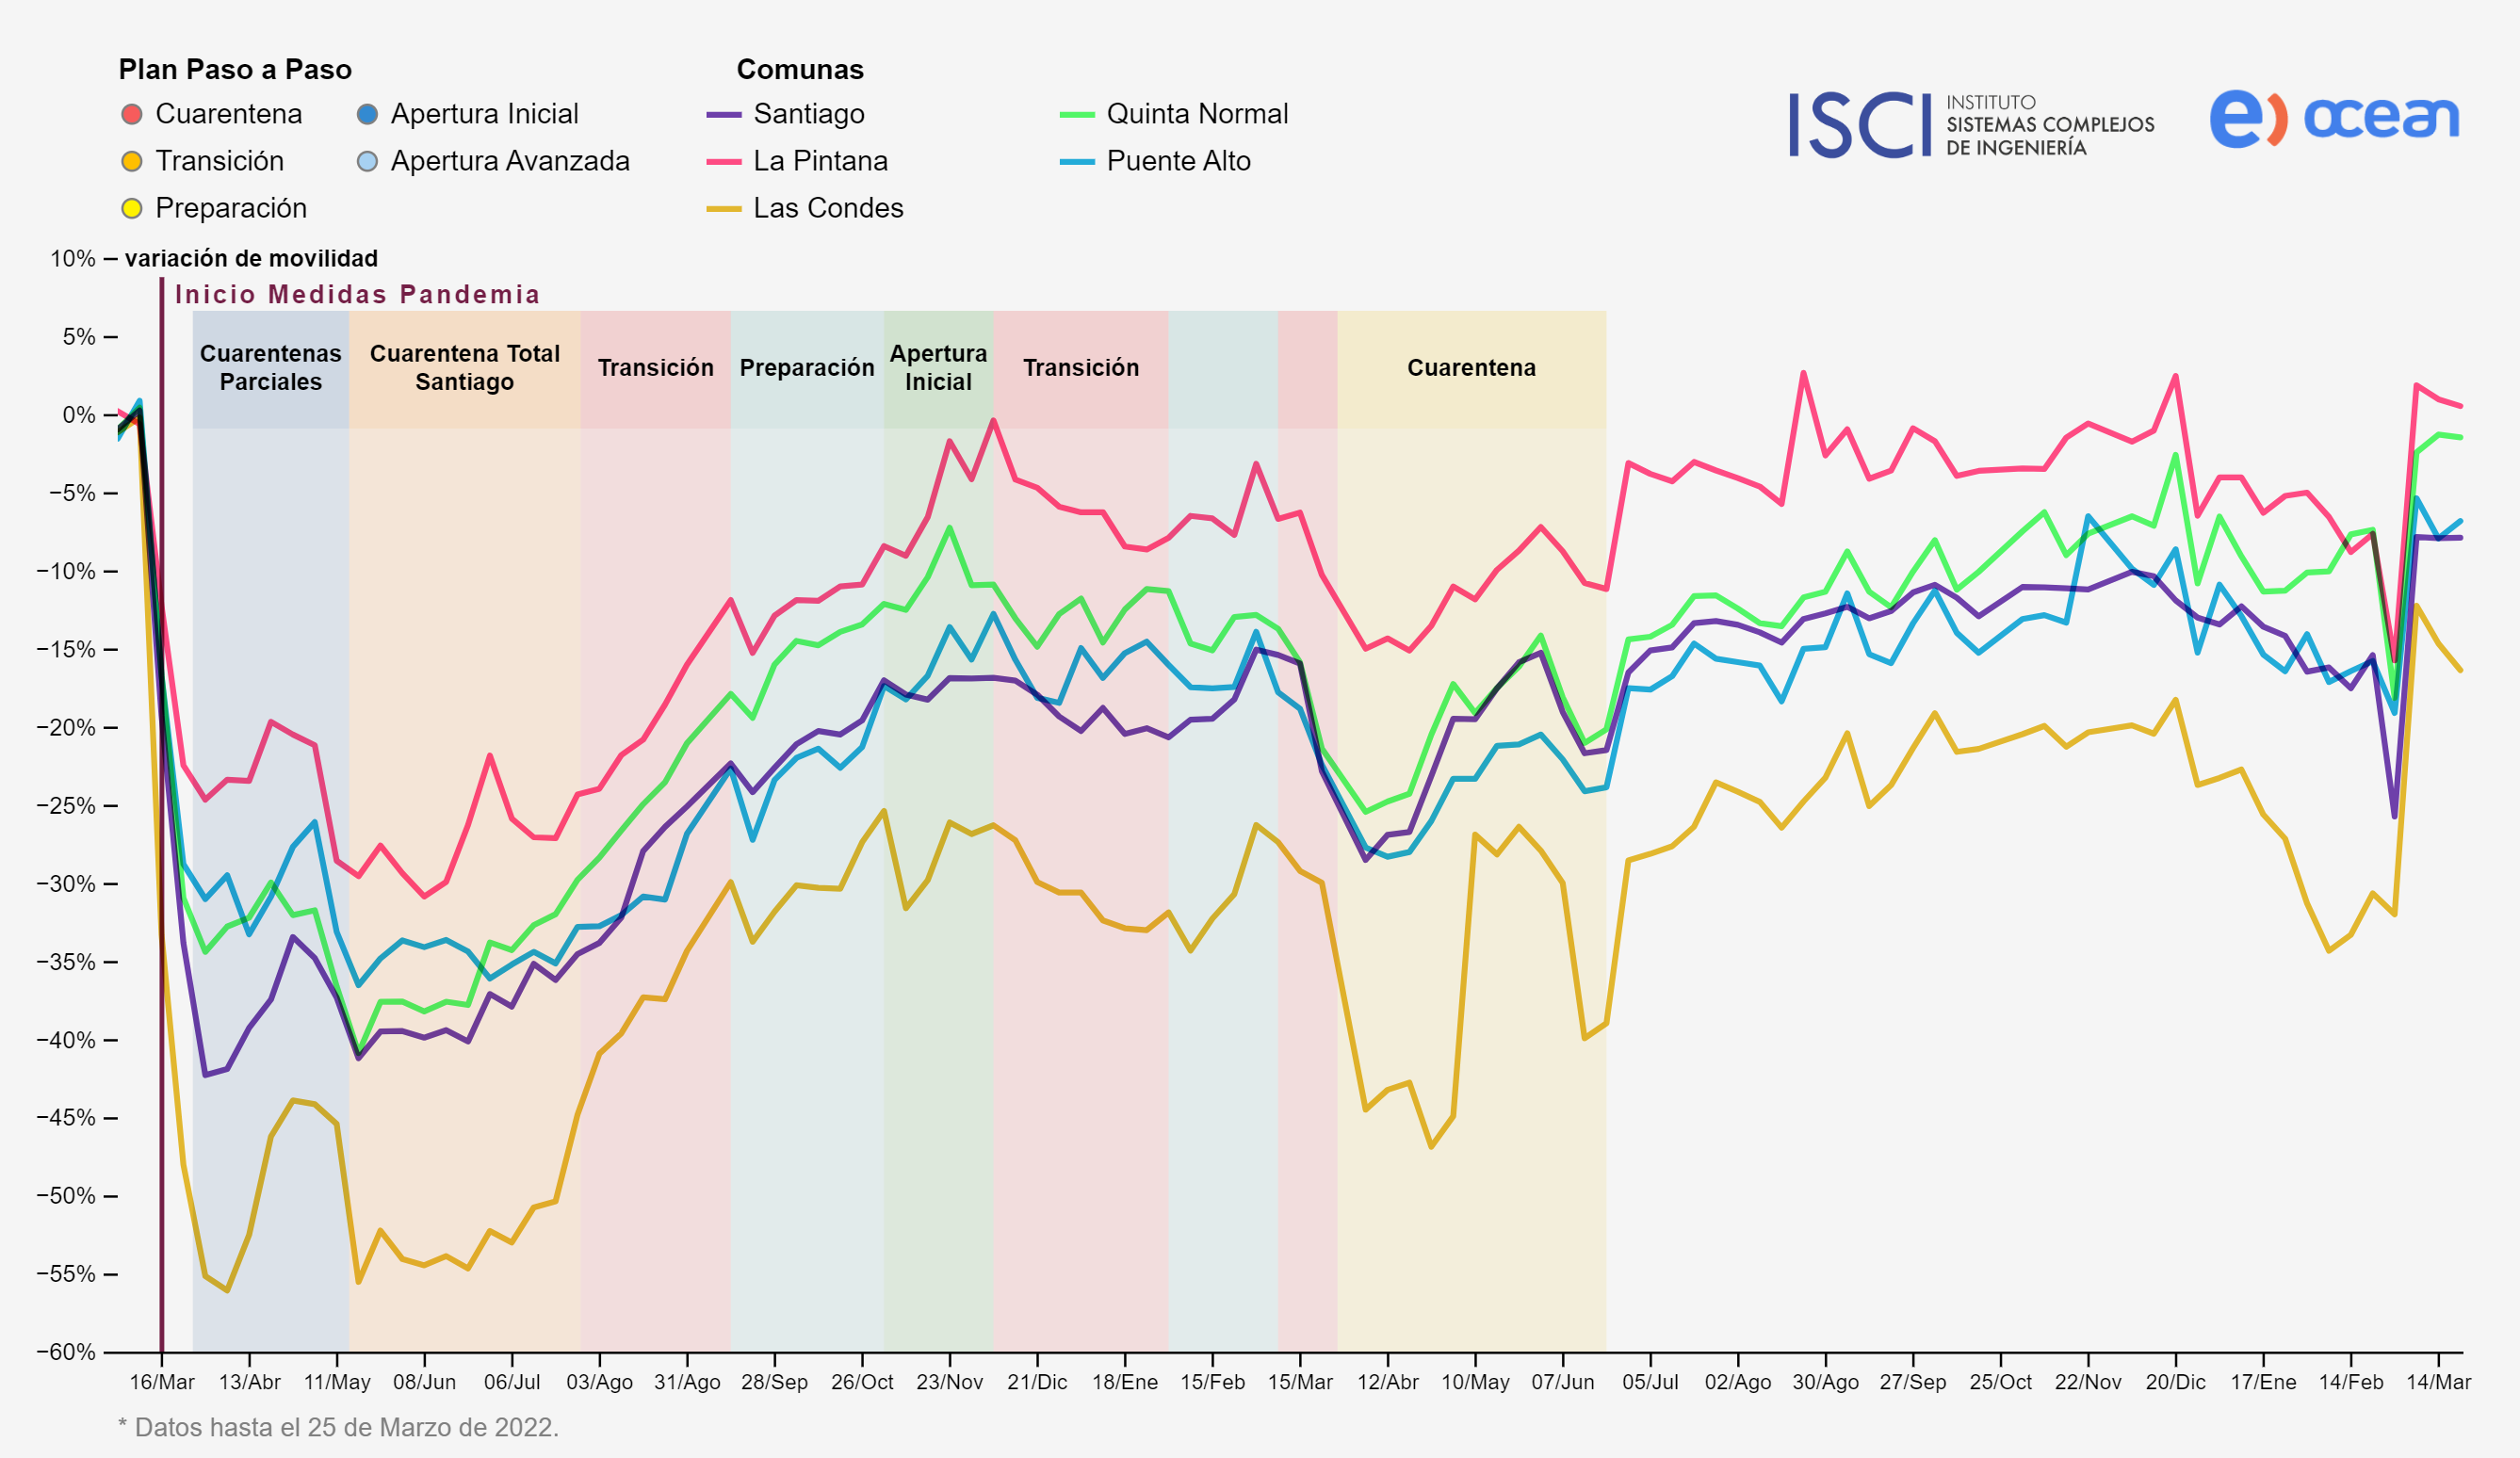
\includegraphics[width=\textwidth]{img/metodologia/datos/movilidad-RM.png}
\caption[Diferencias en la variación de movilidad de cinco comunas de la Región Metropolitana.]{Diferencias en la variación de movilidad de cinco comunas de la Región Metropolitana, desde marzo de 2020 a marzo de 2022. Fuente: ISCI Covid Analytics.}
\label{img:ISCI-movilidad-RM-1}
\end{figure}

La metodología será puesta a prueba estudiando el desarrollo de la pandemia por COVID-19 en la ciudad de Santiago de Chile. Ya desde el comienzo de la pandemia en Santiago, \cite{Olivares2020} hacía notar las dificultades de las clases socioeconómicas más bajas para cumplir las cuarentenas. Esto puede verse claramente en la figura \ref{img:ISCI-movilidad-RM-1}; comunas más acomodadas como Las Condes y Vitacura tienen una reducción de movilidad superior a comunas con menos recursos como La Pintana, a lo largo de toda la pandemia. Varios estudios \cite{Mena2021}\cite{Bennett2021}\cite{Gozzi2021} han notado las significativas diferencias en el impacto de la pandemia en los distintos sectores socioeconómicos de la capital del país, atribuyéndolas, entre otros factores, a la capacidad de cumplimiento de las cuarentenas y las diferencias en el acceso a salud.

Además de lo anterior, el Ministerio de Ciencia, Tecnología, Conocimiento e Innovación de Chile ha hecho disponibles públicamente \cite{MINCIENCIA} varias series de datos epidemiológicos de casos infectados confirmados, hospitalizados, hospitalizados UCI, fallecidos, vacunados, etc. Estos datos poseen diversos niveles de segregación, por comuna, edad o sexo. Todas estas características hacen de la ciudad de Santiago un buen escenario escenario donde implementar el modelo.




\section*{Objetivos}

El objetivo principal del trabajo es estimar el factor sanitario de distintas clases sociales, por medio del \textit{framework} lagrangiano de clases y ambientes de \cite{Bichara2018}. Este objetivo se descompone en dos objetivos específicos. En primer lugar, se necesita definir una metodología que permita estimar el factor sanitario. En segundo lugar, se debe implementar y evaluar la metodología, aplicándola al caso de estudio: la pandemia de COVID-19 en Santiago. 

Definir la metodología requiere plantear el modelo lagrangiano, haciéndole los ajustes necesarios al planteado por \cite{Bichara2018} y considerando las características del COVID-19. Se debe además definir cómo estimar la matriz de tiempos de residencia en base a los datos disponibles. Finalmente, es necesario elegir la variante de filtro de Kalman específica a utilizar en la estimación de parámetros. La implementación requiere de la obtención de datos, el cálculo de la matriz de tiempos de residencia, y la escritura del código para el modelo y el filtro de Kalman.

% Idealmente:
% Este trabajo busca poner a prueba el modelo propuesto en \cite{Bichara2015}, mediante su aplicación al estudio de la evolución de la pandemia de COVID-19 en la ciudad de Santiago de Chile. 
% la idea es que ya no se necesitan las interacciones en cada clase. % Pero a cambio necesito saber en qué ambientes está la gente. 
% De verdad me estoy preguntando qué pasa si solo lo dejo con dos ambientes. Siento que puedo dejarlo con hogar y fuera del hogar. Eso me permitiría meter casi directamente la información de movilidad. Creo que lograría tener movilidad por nivel socioeconómico, en base a la info por comunas. Pero la movilidad por edad creo que está harto más difícil de determinar. 

% Poner a prueba en qué? Bajo qué criterios? El principal criterio es que no necesito conocer cómo interactúa la gente, quiero tener resultados interesantes sin necesariamente saber de qué forma se mezclan todos.

% Cómo puedo evaluar? Comparando la cercanía con los resultados obtenidos con algún otro modelo multiclase?  

%El objetivo general de este trabajo es implementar el \textit{framework} lagrangiano multiclase con dispersión virtual presentado por \cite{Bichara2018}, 

% ... La idea que tengo es... este modelo es lagrangiano, y dice que apaña para evitar tener que calcular las tasas de contacto específicas entre clases, es difícil saber cómo se relaciona la gente... y las opciones que hay son encuestas no necesariamente aplicables. La alternativa presentada es ...

% Una vez que tenemos esa opción...

%Más específicamente, y utilizarlo en la estimación del impacto de las medidas de contención del COVID-19 en la ciudad de Santiago de Chile. 

% Modelos multiclase en Santiagooooo, estoy segura de que hay gente haciendo eso, la fundación ciencia y vida estaba trabajando con un modelo de todas las comunas, haciendo algo parecido a lo que hacía yo pero mucho más complejo. 


% Siempre deben ser verbos terminados en -ar -er -ir 
% Mi objetivo es implementAR el modelo ... qué acciones hay que cumplir 
% \begin{itemize}
% \item Qué compartimientos usar? 
% \item Qué clases elegir? 
% \item Qué ambientes elegir? <-
% \item Cómo formo la matriz de tiempos de residencia, de dónde obtengo los datos? 
% \item Cómo actualizo esa matriz, ya que ha ido cambiando en el tiempo. 
% \item Cómo elijo los parámetros para ajustarlo a los datos existentes de avance de la pandemia? Qué dejo constante? Qué dejo variable? Qué método uso para los constantes? 
% \item Cómo evalúo lo bien que funciona el modelo?
% \end{itemize}

% - Elección del modelo. Esto aún tengo que discutirlo... pero incluye: qué clases usar, que compartimientos usar, cuántos ambientes, etc.
% - Datos disponibles: EOD, datos de movilidad comunal, datos de movilidad de Google por ambiente. Esto para la matriz de 
% - Metodologías dependen de cada objetivo específico 
% - Ajuste del modelo: datos que le voy a dar para ajustar. De qué forma ajusto. 
% - Datos que usaré para verificación, pa cachar qué tan bien funciona la cuestión. 


 

\section*{Metodología}

Para cumplir los objetivos antes expuestos se lleva a cabo la siguiente metodología, la cual se divide en varias etapas. En primer lugar, es necesario explorar las distintas fuentes de datos disponibles, tanto de movilidad y viajes como las series de tiempo epidemiológicas, como cantidad de casos registrados, fallecidos, etc. Esto permite decidir el modelo específico a utilizar, lo que incluye la elección de compartimientos a utilizar (susceptibles, expuestos, infectados, etc), parámetros, además de las clases y ambientes. Todo esto debe considerar las características del COVID-19 y también los datos disponibles. 

Una vez decididas las clases y ambientes, es necesario estimar una matriz de tiempos de residencia, que diga cuánto tiempo pasa cada clase en cada lugar. Se desea que esta matriz sea variable en el tiempo, de forma que incorpore cambios en la movilidad causados por las medidas de mitigación, como cuarentenas, teletrabajo, etc.

Todo lo anterior ya permite correr un modelo de la ciudad de Santiago, definiendo factores sanitarios sintéticos y obtener simulaciones. Se busca ahora estimar el factor sanitario a partir de observaciones del modelo. Para esto se utiliza Filtro de Kalman, y es necesario elegir e implementar una de sus muchas variantes (extendido, \textit{unscented}, filtro por ensambles, etc), y elegir cómo usar el filtro para hacer estimación de parámetros (estado aumentado, filtro de Kalman con múltiples modelos, etc).

Posteriormente se estiman los factores sanitarios para cada una de las clases elegidas, ajustando el modelo a los datos reales de la ciudad de Santiago. Para esto es necesario definir qué variables del modelo observar, que datos utilizar como observación y cómo ajustar los parámetros específicos del filtro.

Finalmente, se utiliza la matriz de tiempos de residencia y los factores sanitarios obtenidos para generar varios casos hipotéticos; distintas variaciones en cuarentenas, diferentes niveles de cuidado. Esto entrega varios desarrollos hipotéticos de la pandemia, y se usará para evaluar el modelo.


\section*{Contribuciones y trabajos relacionados}

A continuación se describen las principales contribuciones de este trabajo. En primer lugar, la propuesta de una metodología que permite estudiar las medidas de cuidado de forma independiente a la movilidad. En segundo lugar, la aplicación del \textit{framework} lagrangiano de clases y ambientes presentado por \cite{Bichara2018} a un caso de estudio, lo cual no había sido hecho con anterioridad. Este trabajo guarda, sin embargo, cierta similitud con \cite{Shikhmurzaev}, que plantea un modelo que incorpora patrones de actividad.

En tercer lugar, la implementación en Matlab de la técnica propuesta por \cite{Munizaga2011} de obtención de uso del tiempo partir de los viajes de una Encuesta Origen-Destino. Esta implementación es de código abierto y se encuentra isponible en el repositorio \url{https://github.com/tabitaCatalan/lagrangian-time}. Se utilizan datos de la Encuesta Origen-Destino Santiago 2012.

En cuarto lugar, el desarrollo de una librería, escrita en el lenguaje Julia, para el trabajo con Filtro de Kalman con dinámica y observadores lineales y/o no lineales. Esta se encuentra documentada, es extensible y de código abierto. Está disponible en el repositorio \url{https://github.com/tabitaCatalan/kalman}. Existen librerías similares en el mismo lenguaje como KalmanFilters.jl y Kalman.jl, pero estas no fueron usadas debido a que en la etapa de decidir qué Filtro utilizar, ninguna contaba con todas las opciones que se quería explorar. 

En quinto lugar, el planteamiento de una metodología para el ajuste de los hiperparámetros relacionados a la covarianza del filtro de Kalman, al estimar parámetros de un modelo epidemiológico. Este era un vacío en trabajos como \cite{Hasan2020} y \cite{Sameni2020}, donde se limitan a elegir un valor fijo para el caso particular que trabajan, sin ofrecer una justificación.

Finalmente, la aplicación del modelo al desarrollo de la pandemia de COVID-19 en la ciudad de Santiago de Chile, lo que permite una estimación de la vulnerabilidad/factor sanitario, de forma independiente a la movilidad. Modelos anteriores de Santiago como \cite{Gozzi2021} solo consideran movilidad.


\section*{Estructura de la tesis}
El resto de esta tesis está organizado como sigue. El capítulo \ref{chap:marco} establece las bases para entender el trabajo realizado. Se presentan varios conceptos relevantes de modelos epidemiológicos y de la teoría de filtro de Kalman. Se exponen también los antecedentes del caso de estudio; la enfermedad COVID-19 y su desarrollo en la ciudad de Santiago de Chile.

El capítulo \ref{chap:metod} justifica y detalla los procedimientos seguidos; cómo se usó el framework de \cite{Bichara2018}, los datos utilizados, los supuestos y simplificaciones hechas, el modelo final utilizado y las técnicas específicas implementadas.

El capítulo \ref{chap:results} presenta los principales resultados obtenidos; la matriz de tiempos de residencia, el caso sintético utilizado para ajustar los parámetros del filtro de Kalman y las estimaciones para el factor sanitario obtenidas utilizando datos reales. Se muestran también los diferentes escenarios hipotéticos generados a partir de esas estimaciones.

El capítulo \ref{chap:discus} discute los resultados obtenidos para el caso de estudio, sus implicaciones y limitaciones. Comenta además el  \textit{framework} lagrangiano planteado en \cite{Bichara2018}, sus ventajas y dificultades a la hora de implementarlo. Se plantean posibles extensiones y trabajo futuro.



\end{intro}
%%%%% ESTABLECER QUE EL NIVEL SOCIOECONOMICO NO QUEREMOS DEJARLO FUERA

%%%%%%%%%%%%%%%%%%%%%%%%%%%%%%%%%%%%%%%%%%%%%%%
% Indice 
%%%%%%%%%%%%%%%%%%%%%%%%%%%%%%%%%%%%%%%%%%%%%%%
% Enfermedades contagiosas y la amenaza que suponen. % Esto habla de la importancia del tema.
% Modelos epidemiológicos en general 
%\include{1-1-modelosepi}
% El modelo que nos interesa. También decir por qué es interesante y de qué limitaciones intenta hacerse cargo.
%\include{1-2-virtualdispersal}
% Con todo eso de arriba estoy estableciendo y delimitando mi territorio. 

% Ahora establezco mi nicho 
% El modelo no ha sido utilizado con datos reales ... blah blah 



